%% Graph-CoLD -- SpringerOpen Cybersecurity submission (DOUBLE-ANONYMOUS review copy)
%% Generated from graph_cold_cas_final.tex (content identical; format + anonymity only).
%% Class: Springer Nature sn-jnl (sn-basic numbered reference style).
%% Anonymity: no author names/affiliations/emails; repository links withheld until
%% acceptance. Per the journal's instructions, ALL Declarations (incl. Availability
%% of data and materials) appear ONLY in the separate title page file
%% (title_page_sn.tex), which also carries the full author metadata.
\documentclass[pdflatex,referee,lineno,sn-basic,Numbered]{sn-jnl}

\usepackage{amsmath,amssymb}
\usepackage{graphicx}
\graphicspath{{./}{../../figures/}}
\usepackage{booktabs}
\usepackage{multirow}
\usepackage{xcolor}
\usepackage{tikz}
\usetikzlibrary{positioning,arrows.meta}
\newcounter{algorithm}
\renewcommand{\thealgorithm}{\arabic{algorithm}}
\hypersetup{hidelinks}

\raggedbottom

\begin{document}

\title[When Does Graph Structure Help Noisy-Label IDS?]{When Does Graph Structure Help Noisy-Label Intrusion Detection?
A Leakage-Audited Study of Rare-Class Training-Signal Retention}

\abstract{Noisy-label training pipelines can discard low-frequency samples that
carry much of the learnable signal for rare classes. We study whether a
multi-view graph consistency diagnostic and soft sample weighting retain that
signal without treating benchmark rows as operational or forensic evidence. We
extend CoLD with Graph-CDM, a label-space diagnostic over the graph views
supported by each dataset, and compare soft weighting with a shared-pipeline
hard-deletion ablation. Experiments use CICIDS-2017 and UNSW-NB15 for
intrusion-detection classification; CESNET-TLS-Year22 is explicitly included as
a long-tail TLS service-classification stress test, not as an attack dataset.
Under the current leakage-audited protocol, Graph-CDM's aggregate Macro-F1 gain
over CoLD is dataset dependent: it is largest on CICIDS-2017 and at most $+0.01$
on the other two datasets. Under 40--80\% asymmetric training-label noise, soft
weighting improves Tail-F1 over hard deletion by $+0.073$, $+0.022$, and $+0.040$
on CICIDS, CESNET, and UNSW, respectively; no statistically significant aggregate
Macro-F1 difference was detected by the current analysis. Confident Learning
outperforms Graph-CoLD on aggregate and tail metrics on all three datasets. A
leakage audit further shows that exact duplicates (24\% of CICIDS-2017 training
rows) and clean-label paths can substantially inflate graph-denoising results.
The supported claim is therefore mechanism-level and bounded: soft retention can
preserve rare-class training signal within this synthetic-noise benchmark
pipeline, but it is neither a universal accuracy improvement nor evidence of SOC
or forensic effectiveness.}

\keywords{intrusion detection, noisy labels, graph learning,
training-signal retention, leakage audit, rare-class robustness}

\maketitle

\section{Introduction}
\label{sec:intro}
Machine-learning classifiers underpin modern network intrusion-detection systems
(IDS) and security operations centers (SOCs). These models are trained from labels
that are seldom perfect: they may be delayed, produced by rules of uneven quality,
or shaped by analyst workflows that emphasize high-severity cases~\cite{arp2022dodont,song2022survey}.
The resulting label noise degrades both detection quality and operational triage.
Crucially, the cost of label noise is asymmetric. Discarding a mislabeled benign
flow may raise a benchmark score, but discarding an informative low-frequency
sample can remove much of the training signal available for a rare class.

This asymmetry motivates a reframing of the problem. Conventional noisy-label
pipelines treat suspicious samples as contamination to be purged; we instead
treat data curation as a \emph{training-signal retention} problem, in which the
decision to delete weighs estimated label unreliability against the class-level
cost of losing scarce training examples. This is a mechanism-level learning
claim: benchmark rows are not, by themselves, SOC investigation or forensic
evidence. The question is therefore not only \emph{how accurately} noise can be
detected, but \emph{what should be done} with samples the detector cannot
confidently classify: delete, trust, or retain at reduced influence.

CoLD~\cite{yang2026cold} recently framed noisy-label IDS through \emph{local
consistency}: because different traffic classes can share feature neighborhoods,
label noise induces spurious associations, and a collaborative representation can
identify and remove likely-noisy samples before training. CoLD, like most
dataset-purification methods, ultimately performs \emph{hard deletion}. We take
CoLD as our baseline and ask two questions. (Q1) Does lifting the diagnostic from
independent samples to a multi-view graph, kept strictly in label space, improve
robustness? (Q2) Does replacing hard deletion with signal-preserving soft
weighting---which down-weights rather than deletes suspicious-but-informative
samples---retain rare-class training signal and improve tail-class detection?

Answering these questions honestly required an unusual amount of methodological
hygiene. Our first implementations produced spectacular gains that did not
survive scrutiny: a leakage audit revealed that (i) CICIDS-2017 contains 24\%
exact-duplicate records that let neighborhood consistency trivially recover
labels, and (ii) any use of clean-label signal in the scoring or graph
construction inflates results. After removing both, the apparent advantage shrank
to a modest, defensible level, and the headline metric we had used for signal
retention turned out to be tautological. We report this process because it is, we
believe, a contribution in its own right: graph-based denoising results in
security are easy to inflate and must be audited.

\paragraph{Contributions.}
The current empirical record supports the following bounded contributions:
\begin{enumerate}
\item A \emph{leakage audit} that quantifies duplicate- and clean-label-path
inflation and documents how apparently large graph-denoising gains can collapse
under a de-oracled protocol (Section~\ref{sec:res-leak}).
\item A \emph{signal-preserving soft weighting} rule that improves Tail-F1 over
hard deletion under high asymmetric noise within an otherwise shared pipeline
(Section~\ref{sec:res-tail}). The result concerns rare attack classes on
CICIDS/UNSW and low-frequency service classes on CESNET; the current aggregate
analysis detects no significant difference but does not establish equivalence.
\item Graph-CDM, a \emph{label-space} multi-view consistency diagnostic used to
study when graph structure helps. Its aggregate gain over CoLD is modest and
dataset dependent, and the three-dataset informativeness pattern is descriptive,
not inferential (Sections~\ref{sec:res-aggregate} and~\ref{sec:res-info}).
\end{enumerate}
We deliberately bound our claims. Graph-CoLD is not a universal accuracy
improvement, and retained benchmark samples are not operational evidence. Its
distinctive mechanism-level value is retaining rare-class training signal that
hard deletion can discard.

\section{Related Work}
\label{sec:related}
\paragraph{Noisy-label learning.}
Approaches divide into robust-training and dataset-purification families. Robust
training modifies losses or training dynamics: loss correction with a transition
matrix~\cite{patrini2017making}, peer-network small-loss selection
(Co-teaching~\cite{han2018coteaching}, Co-teaching+~\cite{yu2019coteachingplus}),
disagreement-based updates (Decoupling~\cite{malach2017decoupling}), and
semi-supervised treatment of suspected-noisy data
(DivideMix~\cite{li2020dividemix}). Purification detects and removes mislabeled
instances: confident learning~\cite{northcutt2021confident}, representation-based
filtering (FINE~\cite{kim2021fine}), and, in security, MORSE~\cite{wu2023morse}
and MCRe~\cite{yuan2023mcre}. CoLD~\cite{yang2026cold} is the closest prior work
and our baseline. Our departure is twofold: we keep the diagnostic in label space
(avoiding the distance-metric fragility CoLD itself criticizes), and we replace
deletion with signal-preserving weighting motivated by the semi-supervised
insight that suspected-noisy samples carry usable signal~\cite{li2020dividemix,wu2023morse}.

\paragraph{Graph learning for security telemetry.}
Security events are relational, and graph neural
networks~\cite{kipf2017gcn,velickovic2018gat,hamilton2017graphsage,hu2020hgt}
naturally propagate contextual signals. Provenance-graph IDS such as
Flash~\cite{rehman2024flash} and Argus~\cite{xu2024argus} demonstrate the value of
structure for enterprise detection. We use graph representation learning as a
backbone but, unlike embedding-distance denoisers, keep the noise diagnostic in
label space so it stays aligned with the classifier.

\paragraph{SOC alert handling and concept drift.}
Operational systems must also cope with alert volume and distribution shift.
Alert-classification and triage work~\cite{vaarandi2024nids,chavali2024rlalert}
and drift-aware detection~\cite{yang2021cade} motivate our operational framing,
though our contribution is denoising for rare-class signal retention rather than a
deployed triage study.

\paragraph{Contrastive self-supervision.}
Our representation stage uses cross-view contrastive
learning~\cite{chen2020simclr}, adapted so that the same node in two views forms a
positive pair.

% <<P4-RELATED-WORK>>
% BLOCK A -> <<P4-RELATED-WORK>>

\subsection{Positioning and Open Challenges}

\subsubsection*{Noisy-label learning for intrusion detection}

Learning from noisy labels has become an important challenge in security
analytics because network telemetry is often collected through heterogeneous
sources, automated rules, and delayed analyst feedback. Unlike conventional
computer vision benchmarks where label corruption can often be controlled
synthetically, security labels may reflect incomplete attack knowledge,
imbalanced detection rules, and evolving adversarial behaviors
\cite{guerra2022datasets,qing2023lowquality}. Therefore, improving robustness
requires not only higher classification accuracy but also understanding which
samples should be trusted and which samples contain useful but uncertain training signal.

Existing noisy-label learning methods can be broadly divided into robust
training and dataset purification. Robust training approaches attempt to reduce
the influence of corrupted samples during optimization. Loss correction methods
estimate label transition characteristics and modify the training objective
\cite{zhao2021enhancing}. Sample-selection approaches exploit uncertainty,
loss dynamics, or disagreement between models to identify potentially noisy
instances \cite{xia2021sample,liu2021metric}. Co-teaching and related
disagreement-based approaches train multiple networks and exchange selected
small-loss samples to reduce memorization of corrupted labels
\cite{han2018coteaching,yu2019coteachingplus}. Decoupling further separates the
decision of when to update from how to update, demonstrating that disagreement
between classifiers can provide useful information under label corruption
\cite{malach2017decoupling}.

A different family focuses on dataset purification. Confident Learning estimates
label uncertainty by identifying statistically inconsistent annotations
\cite{northcutt2021confident}. FINE explores representation-space filtering of
noisy instances through latent feature structures
\cite{kim2021fine}. In security domains, MCRe and MORSE extend noisy-label
handling toward malicious traffic and malware classification scenarios
\cite{yuan2023mcre,wu2023morse}. More recently, intrusion detection studies
have explored contrastive learning and representation enhancement as a way to
improve robustness against noisy or incomplete observations
\cite{wang2022feco,yue2022cleid}.

CoLD provides the closest foundation for our work by introducing collaborative
label denoising specifically for network intrusion detection. However, existing
purification-oriented methods generally treat suspicious samples as removable
noise. This assumption is problematic for imbalanced classification because
rare-class samples may simultaneously appear inconsistent and be important to
the learned decision boundary.
Graph-CoLD therefore does not aim to replace purification, but instead explores
whether structural context and signal-preserving weighting can retain
informative suspicious instances.

\subsubsection*{Graph learning and contrastive representation for security}

Graph representation learning has become increasingly important for security
analytics because network activities naturally form relational structures among
hosts, addresses, sessions, and temporal events. Graph convolutional networks
and graph attention networks demonstrated that neighborhood information can
improve representation learning when samples are connected through meaningful
relations \cite{kipf2017gcn,velickovic2018gat}. Inductive graph representation
learning further enables scalable modeling of previously unseen nodes
\cite{hamilton2017graphsage}, while heterogeneous graph transformers extend
graph reasoning to multiple relation types \cite{hu2020hgt}.

In security applications, graph methods have mainly focused on attack
detection, provenance analysis, and contextual behavior modeling. Systems such
as Flash demonstrate the value of provenance graph representation learning for
enterprise intrusion detection \cite{rehman2024flash}. Other work investigates
security-oriented representation learning and graph analytics for detecting
suspicious behaviors \cite{xu2024argus}. These approaches usually focus on
discovering malicious structures from graph embeddings.

Graph-CoLD differs from these methods in its objective. The graph structure is
not directly used as an anomaly detector; instead, it provides contextual
signals for a label-space consistency diagnostic. This distinction is
important because embedding distance alone may capture feature similarity while
remaining disconnected from the classifier's final prediction behavior. By
combining graph context with prediction-space disagreement, Graph-CoLD aims to
identify unreliable labels while preserving samples that remain informative.

\subsubsection*{SOC alert triage, prioritization, and concept drift}

Modern SOC environments face not only detection accuracy challenges but also
large-scale alert management problems. Excessive alerts, evolving attack
behaviors, and changing network distributions create operational pressure for
analysts. Alert classification and active-learning approaches have explored
ways to reduce analyst workload by improving alert categorization
\cite{vaarandi2024nids}. Reinforcement-learning-based alert prioritization
methods further investigate how automated systems can rank alerts according to
operational importance \cite{chavali2024rlalert}.

Beyond static classification, concept drift has become a critical challenge in
long-running security monitoring. Detection systems must adapt when normal
traffic patterns, attack strategies, and service behaviors evolve. Studies such
as CADE, RecDA, and Insomnia investigate drift detection and adaptation
mechanisms for network intrusion detection
\cite{yang2021cade,yang2024recda,andresini2021insomnia}. Recent SOC-oriented
research also explores alert aggregation and filtering through deep learning
models to improve investigation efficiency
\cite{liu2025deepdrac,shon2023semisup,wang2024alertagg}.

These operational studies motivate our security framing, but Graph-CoLD
addresses a different layer of the problem. Rather than replacing analyst
triage or predicting attack priority directly, we focus on improving the
quality of the training data that supports downstream detection. The key
difference is that Graph-CoLD combines three principles: label-space
consistency diagnosis, signal-preserving retention, and leakage-audited
evaluation. This design aims to answer when graph-based denoising genuinely
helps security analytics and when structural information is insufficient.
\section{Problem Formulation}
\label{sec:problem}
Let $V$ be the set of training flows and $\mathcal{M}$ the set of \emph{active}
graph views. Each view $m\in\mathcal{M}$ induces a graph $G^{m}=(V,E^{m})$ over the
same nodes. The observed training label $\tilde{y}_v$ may differ from the
unobserved clean label $y_v$. We seek a classifier that (i) resists the effect of
noisy labels, and (ii) retains useful training signal---especially clean samples
of rare classes that a purifier is tempted to discard.

We adopt three design principles. First, the noise diagnostic operates in
\emph{label/prediction space}, not embedding distance, so it remains aligned with
the classifier and does not re-introduce the local-consistency fragility of
distance-based purifiers. Second, denoising is \emph{signal preserving}: a
suspicious but informative sample is down-weighted rather than removed. Third, the
evaluation is traceable to audited real data, with explicit scope limits.

\section{Method}
\label{sec:method}
Graph-CoLD is a two-stage extension of CoLD: self-supervised multi-view
representation learning, followed by a label-space consistency diagnostic that
drives a signal-preserving weight (Figure~\ref{fig:overview}).

\begin{figure}[t]
\centering
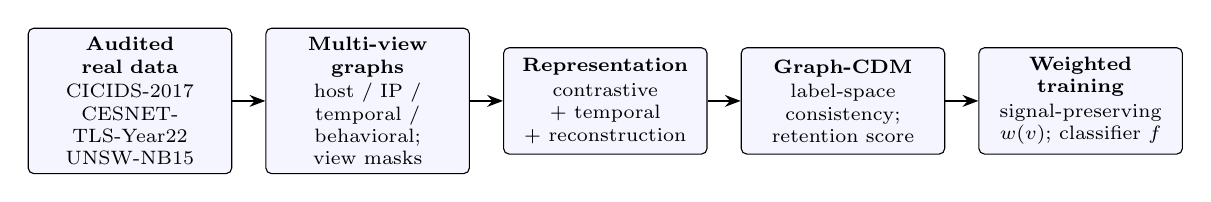
\begin{tikzpicture}[
  stage/.style={draw, rounded corners=2pt, align=center, minimum height=1.35cm,
    text width=2.35cm, font=\scriptsize, fill=blue!4},
  arr/.style={-{Stealth[length=2mm]}, thick},
  node distance=0.42cm]
\node[stage] (data) {\textbf{Audited real data}\\[1pt]
CICIDS-2017\\CESNET-TLS-Year22\\UNSW-NB15};
\node[stage, right=of data] (views) {\textbf{Multi-view graphs}\\[1pt]
host / IP / temporal /\\behavioral; view masks};
\node[stage, right=of views] (rep) {\textbf{Representation}\\[1pt]
contrastive + temporal\\+ reconstruction};
\node[stage, right=of rep] (cdm) {\textbf{Graph-CDM}\\[1pt]
label-space consistency;\\retention score};
\node[stage, right=of cdm] (out) {\textbf{Weighted training}\\[1pt]
signal-preserving\\$w(v)$; classifier $f$};
\draw[arr] (data) -- (views);
\draw[arr] (views) -- (rep);
\draw[arr] (rep) -- (cdm);
\draw[arr] (cdm) -- (out);
\end{tikzpicture}
\caption{Graph-CoLD pipeline. Only views supported by a dataset's verified schema
are activated; unsupported views are disabled rather than fabricated. The
consistency diagnostic (Graph-CDM) is computed in label space and feeds a
signal-preserving soft weight and a downstream classifier. Datasets are
CICIDS-2017, CESNET-TLS-Year22, and UNSW-NB15 (active views vary by dataset;
see Table~\ref{tab:data}).}
\label{fig:overview}
\end{figure}

\subsection{Multi-view graph construction}
Views are built from semantically related feature blocks over the training nodes:
a \emph{host} view links samples sharing endpoint identifiers; an \emph{IP} view
uses communication/flow statistics, ports, protocol and TLS metadata; a
\emph{temporal} view links samples within a time window; a \emph{behavioral} view
groups service, protocol, port-state, and related behavioral feature blocks
(it is a feature-block view, not host-process lineage) and is used only where such
fields exist. Support is part of the reproducible
dataset contract: CICIDS-2017 activates host/IP/temporal, CESNET-TLS-Year22
activates IP/temporal, and UNSW-NB15 activates temporal/behavioral. Threat-intelligence
views are disabled when the fields are absent. Crucially, edges never cross the
train/test split, and (Section~\ref{sec:res-leak}) exact/near-duplicate edges are
removed.

\subsection{Self-supervised representation}
Each active view produces a node embedding $z_v^{m}$ from Bernoulli-masked input
features, $x'_v = x_v \odot \mathrm{Bernoulli}(1-\delta)$. Cross-view contrastive
learning treats the same node in two views as a positive pair and other batch
nodes as negatives:
\begin{equation}
\mathcal{L}_{\text{con}} = -\log
\frac{\exp(\mathrm{sim}(z^{a}_v,z^{b}_v)/\tau)}
{\sum_{u}\exp(\mathrm{sim}(z_v,z_u)/\tau)} .
\end{equation}
Temporal alignment and reconstruction terms regularize the embedding,
$\mathcal{L}_{\text{rep}}=\mathcal{L}_{\text{con}}+\alpha\mathcal{L}_{\text{temporal}}
+\beta\mathcal{L}_{\text{recon}}$; active views are fused by mean aggregation to
obtain $z_v$.

\subsection{Graph-CDM: a label-space consistency diagnostic}
For each node $v$,
\begin{equation}
\mathrm{GraphCDM}(v)=\lambda_1 D_{\text{pred}}(v)+\lambda_2 D_{\text{neigh}}(v)
+\lambda_3 D_{\text{view}}(v)+\lambda_4 D_{\text{chain}}(v),
\end{equation}
where the prediction term compares per-view predicted labels with the observed
\emph{noisy} training label,
\begin{equation}
D_{\text{pred}}(v)=\frac{1}{M}\sum_{m=1}^{M}\mathbf{1}[\tilde{y}^{m}_v\neq \tilde{y}_v],
\end{equation}
the neighborhood term is a label-space KL divergence between a node's soft
prediction and its neighborhood mean,
$D_{\text{neigh}}(v)=\mathrm{KL}\!\big(\hat{y}_v \,\|\,
|N(v)|^{-1}\sum_{u\in N(v)}\hat{y}_u\big)$,
and the view term measures active-view mode disagreement,
$D_{\text{view}}(v)=1-\max_c\frac1M\sum_m\mathbf{1}[\tilde{y}^{m}_v=c]$.
$D_{\text{chain}}$ is reserved for verified provenance/temporal chains and is not a
driver of the reported results. No term uses clean labels or the noise mask;
this is enforced by a regression test.

\subsection{Signal-preserving soft weighting}
The internal evidence score protects samples that would be costly to discard,
$e(v)=\text{freq\_protect}(\tilde{y}_v)\,(1+\gamma\,\text{anom}(v))$, min-max
normalized to $\tilde{e}(v)$. Rather than a small additive floor (which collapses
to hard deletion), we use an evidence-\emph{rescue} form so that suspicious yet
high-evidence samples retain real weight:
\begin{equation}
w(v)=\underbrace{\sigma\!\big(-\kappa(\mathrm{GraphCDM}(v)-\theta)\big)}_{\text{clean branch}}
+\underbrace{\big(1-\sigma(\cdot)\big)\,\lambda_{r}\,\tilde{e}(v)}_{\text{evidence rescue}} .
\end{equation}
The classifier minimizes $\sum_v w(v)\,\mathrm{CE}(f(z_v),\tilde{y}_v)$. Setting
$\lambda_r=0$ and thresholding recovers hard deletion; this is our
\texttt{ablation\_hard} comparator, sharing the identical graph, representation,
and diagnostic so that the ablation isolates \emph{only} the weighting.

We stress the intended interpretation of this internal score: ``evidence'' here
means a heuristic estimate of training-signal retention value, not SOC or
forensic evidence. Frequency protection encodes \emph{deletion cost}, not
trustworthiness. A rare sample is protected because discarding it is costly---it
may be one of few training examples for a tail class---not because rarity implies
a clean label.
The score is thus a heuristic proxy for a risk-aware retention signal
$R_{\text{delete}}(v)\propto \mathrm{Cost}(\tilde{y}_v)\,\big(1+\gamma\,\text{anom}(v)\big)$,
where $\mathrm{Cost}$ is high for rare classes, and the weighting in
Eq.~(4) implements risk-aware sample retention: samples with high diagnostic
suspicion but high deletion cost keep reduced---never zero---influence.
A full decision-theoretic treatment that models
$P(\text{clean}\mid x)\cdot\mathrm{Cost}(y)$ explicitly is left to future work;
the empirical ordering in Section~\ref{sec:res-tail}, where
confident-learning-precision pruning outperforms our heuristic, indicates the
value of sharpening the $P(\text{clean}\mid x)$ component.
Both the aligned CoLD baseline and the \texttt{ablation\_hard} variant use the
same shared encoder architecture, training budget, and view-masking configuration
as Graph-CoLD; they differ only in the presence or absence of graph views and the
weighting rule applied after Graph-CDM scoring.

\subsection{Triage-oriented benchmark proxy}
A priority score $P(v)=\alpha_1\hat{y}_{\text{mal}}(v)+\alpha_2\mathrm{GraphCDM}(v)
+\alpha_3\tilde{e}(v)$ models a triage-oriented ranking. We evaluate it only by
benchmark labels and, as we show, Graph-CoLD ties strong peers on top-$K$
precision; without an analyst study, we claim neither a ranking advantage nor
operational effectiveness.

% <<P4-METHOD-ALGORITHM>>
% BLOCK B -> <<P4-METHOD-ALGORITHM>>

\subsection{Graph-CoLD Optimization Procedure}

The complete Graph-CoLD pipeline consists of representation learning,
label-space consistency estimation, retention scoring, and weighted classifier
optimization. Algorithm~\ref{alg:graphcold} summarizes the complete procedure.

\begin{center}
\refstepcounter{algorithm}\label{alg:graphcold}
\begin{minipage}{0.92\linewidth}
\textbf{Algorithm~\thealgorithm: Graph-CoLD signal-preserving noisy-label learning.}

\textit{Input:} Multi-view graphs $\{G_m\}_{m=1}^{M}$, noisy labels
$\tilde{Y}$, feature matrix $X$. \\
\textit{Output:} Trained classifier $f$.

\begin{enumerate}
\item Construct active graph views according to available telemetry fields.
\item Learn view-specific representations using contrastive, temporal-alignment,
and reconstruction objectives, then fuse them into node embeddings $Z$.
\item Generate prediction-space and neighborhood consistency statistics and
compute a Graph-CDM score for each training sample.
\item Estimate internal retention scores from label frequency and anomaly
factors, then compute the signal-preserving weights $w(v)$.
\item Optimize the classifier using weighted cross entropy and return $f$.
\end{enumerate}
\end{minipage}
\end{center}

The design follows three considerations. First, the diagnostic operates in label
and prediction space rather than pure embedding distance. This maintains
consistency with the classifier decision process and avoids relying solely on
representation similarity. Second, the weighting mechanism adopts an
signal-rescue formulation because suspicious samples may still contain useful
class information. A simple lower bound would approximate hard deletion,
whereas the rescue formulation allows uncertain but informative samples to
participate in training. Third, hard deletion is retained as the primary
ablation because it isolates the contribution of signal preservation while
keeping the same graph representation and diagnostic components.
\section{Experimental Design}
\label{sec:exp}
\subsection{Datasets and protocol}
Table~\ref{tab:data} summarizes three benchmark datasets with different tasks.
CICIDS-2017 and UNSW-NB15 are intrusion-detection datasets. CESNET-TLS-Year22
is a TLS service-classification dataset whose SNI-derived application labels do
not carry attack/benign semantics; we retain it only as a long-tail service-class
stress test and do not use it to support attack-level claims. CICIDS-2017 is used under
an 11-class \emph{post-filter} policy with exact deduplication (24\% of raw
training rows removed; Section~\ref{sec:res-leak}). CESNET-TLS-Year22 is a
year-spanning backbone TLS dataset used under a 25-service-class audit-window policy (it
replaces MALTLS-22, for which we lacked a verified license path). UNSW-NB15 is
used under its partition with the smallest class (Worms) removed. To keep the
study tractable and reproducible we evaluate deterministic audit windows
(train $10{,}000$ / test $5{,}000$); we are explicit that this is a focused study,
not a full-archive evaluation. Noise is injected only into training labels; we
report symmetric, asymmetric, and graph-consistency noise, and for the rare-class
analysis we use asymmetric noise concentrated on tail classes at rates
$\{40,60,80\}\%$ with seeds $0$--$9$. The asymmetric target is benign for the
two IDS datasets and a high-frequency service class for CESNET; legacy result
filenames may use \texttt{tail-to-benign} as an implementation label, but that
term has no semantic meaning for CESNET.

\begin{table}[t]
\centering
\caption{Datasets and active graph views. Source: \texttt{tables/table\_1\_dataset\_protocol.csv}.}
\label{tab:data}
\small
\begin{tabular}{lccc}
\toprule
Dataset & Classes & Sample policy & Active views \\
\midrule
CICIDS-2017 & 11 & post-filter, exact-dedup & host/IP/temporal \\
CESNET-TLS-Year22 & 25 & audit window & IP/temporal \\
UNSW-NB15 & 9 & partition (no Worms) & temporal/behavioral \\
\bottomrule
\end{tabular}
\end{table}

All results in Tables~\ref{tab:main}--\ref{tab:tail} and Figures~\ref{fig:tail}--\ref{fig:info}
are generated by the P2f clean de-oracled runner
(\texttt{reports/p2f\_tighten.md}) on these three datasets; earlier intermediate
result files from D5/D9 used a different protocol and are not cited as final
results.

\paragraph{Reproducibility and statistical protocol.}
The audited data roots are local and are not committed to the repository. Each
dataset uses deterministic audit windows of 10,000 training and 5,000 test
instances. The tail analysis injects asymmetric noise at $\{40,60,80\}\%$ over
seeds 0--9. Paired inference uses 30 like-for-like seed--rate observations per
dataset (ten seeds by three noise rates), with Holm--Bonferroni correction and
bootstrap 95\% confidence intervals. The full command sequence is recorded in
the reproduction commands of \texttt{reports/p2f\_tighten.md}.

\subsection{Baselines and metrics}
We compare Graph-CoLD (soft and semi-supervised variants) with the aligned CoLD
baseline and the \texttt{ablation\_hard} deletion variant across the
Tables~\ref{tab:main}--\ref{tab:tail} result matrix. Two external noisy-label
anchors were run under the \emph{identical} P2f protocol (same audit windows,
splits, seeds, and noise): Confident Learning (cleanlab \texttt{find\_label\_issues}
with a shared-budget ExtraTrees head) and a full Co-Teaching implementation
(dual MLPs with per-batch small-loss co-exchange and a forget-rate schedule
tracking the true injected rate), recorded in
\texttt{results/p5\_external\_baselines.csv} and compared in
Section~\ref{sec:res-tail}. Additional purification
methods (MCRe, MORSE, FINE, Decoupling, and Co-Teaching-lite, a lightweight
approximation superseded by the full implementation above) were evaluated
under an earlier protocol. They were not re-run under the P2f clean-deduplication
protocol and are therefore excluded from Tables~\ref{tab:main}--\ref{tab:tail}
to avoid mixing incompatible result regimes; the MCRe/MORSE fidelity caveat is
documented in \texttt{reports/p2b\_baseline\_fidelity.md}. Metrics reported here
are aggregate Macro-F1, tail-class Macro-F1, tail recall, and paired statistical
comparisons as specified above.

\section{Results}
\subsection{RQ1: A label-space graph diagnostic modestly improves accuracy over CoLD}
\label{sec:res-aggregate}
Table~\ref{tab:main} reports per-dataset means. Graph-CoLD improves aggregate
Macro-F1 over CoLD on all three datasets, with the gain concentrated on CICIDS,
where host/IP/temporal views are most informative, and small on CESNET/UNSW. The
improvements over CoLD are Holm-significant per dataset (CICIDS $p=1.0\times10^{-3}$,
CESNET $p=4.1\times10^{-2}$, UNSW $p=4.1\times10^{-2}$;
source \texttt{tables/table\_p2d\_per\_dataset\_vs\_cold.csv}). Notably,
\texttt{ablation\_hard} already captures most of this gain: the graph and the
label-space diagnostic, not the weighting, drive aggregate accuracy.

\begin{table}[t]
\centering
\caption{Per-dataset mean$\pm$std under high asymmetric tail noise (rates 40/60/80\%,
seeds 0--9; 30 scenarios per dataset). Sources: \texttt{tables/table\_p2f\_summary.csv}
(Graph-CoLD family) and \texttt{results/p5\_external\_baselines.csv} (external anchors,
same protocol). Best value per dataset and metric in bold.}
\label{tab:main}
\small
\begin{tabular}{llccc}
\toprule
Dataset & Method & Macro-F1 & Tail-F1 & Tail-recall \\
\midrule
\multirow{6}{*}{CICIDS-2017}
 & CoLD          & 0.534$\pm$0.039 & 0.047$\pm$0.070 & 0.043$\pm$0.065 \\
 & ablation\_hard & 0.688$\pm$0.087 & 0.361$\pm$0.193 & 0.277$\pm$0.173 \\
 & Graph-CoLD-soft & 0.721$\pm$0.086 & 0.434$\pm$0.191 & 0.328$\pm$0.180 \\
 & Graph-CoLD-semisup & 0.687$\pm$0.093 & 0.357$\pm$0.206 & 0.272$\pm$0.181 \\
 & Confident-Learning & \textbf{0.769$\pm$0.048} & \textbf{0.605$\pm$0.103} & \textbf{0.517$\pm$0.112} \\
 & Co-Teaching & 0.567$\pm$0.071 & 0.118$\pm$0.152 & 0.128$\pm$0.171 \\
\midrule
\multirow{6}{*}{CESNET-TLS-Year22}
 & CoLD          & 0.658$\pm$0.130 & 0.411$\pm$0.247 & 0.306$\pm$0.211 \\
 & ablation\_hard & 0.680$\pm$0.132 & 0.453$\pm$0.249 & 0.331$\pm$0.218 \\
 & Graph-CoLD-soft & 0.692$\pm$0.120 & 0.475$\pm$0.227 & 0.344$\pm$0.204 \\
 & Graph-CoLD-semisup & 0.679$\pm$0.129 & 0.450$\pm$0.243 & 0.327$\pm$0.212 \\
 & Confident-Learning & \textbf{0.805$\pm$0.076} & \textbf{0.708$\pm$0.136} & \textbf{0.628$\pm$0.159} \\
 & Co-Teaching & 0.488$\pm$0.152 & 0.179$\pm$0.258 & 0.181$\pm$0.262 \\
\midrule
\multirow{6}{*}{UNSW-NB15}
 & CoLD          & 0.456$\pm$0.032 & 0.096$\pm$0.068 & 0.187$\pm$0.146 \\
 & ablation\_hard & 0.471$\pm$0.035 & 0.132$\pm$0.077 & 0.205$\pm$0.128 \\
 & Graph-CoLD-soft & 0.485$\pm$0.033 & 0.173$\pm$0.078 & 0.229$\pm$0.120 \\
 & Graph-CoLD-semisup & 0.469$\pm$0.033 & 0.130$\pm$0.074 & 0.194$\pm$0.119 \\
 & Confident-Learning & \textbf{0.499$\pm$0.026} & \textbf{0.254$\pm$0.085} & \textbf{0.317$\pm$0.123} \\
 & Co-Teaching & 0.419$\pm$0.036 & 0.055$\pm$0.080 & 0.120$\pm$0.178 \\
\bottomrule
\end{tabular}
\end{table}

\begin{table}[t]
\centering
\caption{Graph-CoLD vs.\ CoLD Macro-F1 by noise type (mean over noise rates,
seeds 0--9). Source: \texttt{tables/table\_p4\_noise\_type\_breakdown.csv}.}
\label{tab:noisetype}
\small
\begin{tabular}{llrrr}
\toprule
Dataset & Noise type & CoLD & Graph-CoLD-soft & $\Delta$ \\
\midrule
CICIDS-2017 & clean & 0.671150 & 0.778689 & 0.107539 \\
CICIDS-2017 & symmetric & 0.553919 & 0.592429 & 0.038510 \\
CICIDS-2017 & asymmetric & 0.322779 & 0.429941 & 0.107162 \\
CICIDS-2017 & \texttt{graph\_consistency} & 0.496244 & 0.531555 & 0.035311 \\
\midrule
CESNET-TLS-Year22 & clean & 0.966321 & 0.968261 & 0.001941 \\
CESNET-TLS-Year22 & symmetric & 0.898812 & 0.902585 & 0.003774 \\
CESNET-TLS-Year22 & asymmetric & 0.698745 & 0.708302 & 0.009557 \\
CESNET-TLS-Year22 & \texttt{graph\_consistency} & 0.846591 & 0.849355 & 0.002764 \\
\midrule
UNSW-NB15 & clean & 0.494282 & 0.501909 & 0.007627 \\
UNSW-NB15 & symmetric & 0.445324 & 0.445923 & 0.000599 \\
UNSW-NB15 & asymmetric & 0.296512 & 0.303933 & 0.007421 \\
UNSW-NB15 & \texttt{graph\_consistency} & 0.434276 & 0.436233 & 0.001957 \\
\bottomrule
\end{tabular}
\end{table}
% <<P4-RESULTS-NOISETYPE>>
% BLOCK C -> <<P4-RESULTS-NOISETYPE>>

\subsection{Performance under Different Noise Types}

To better understand when Graph-CoLD provides benefits, we analyze performance
across different label-noise mechanisms. Table~\ref{tab:noisetype} summarizes
Macro-F1 results under clean, symmetric, asymmetric, and graph-consistency
noise.

The results show that the benefit of Graph-CoLD is strongly dataset-dependent.
On CICIDS-2017, where host, IP, and temporal relations provide richer structural
signals, Graph-CoLD achieves consistent improvements over CoLD across all noise
types. Under asymmetric noise, the improvement is 0.107 in Macro-F1. This
observation is consistent with the hypothesis that graph context is more
valuable when corruption is associated with non-uniform class behavior.

For CESNET-TLS-Year22 \cite{hynek2024zenodo}, the improvement is smaller because
the baseline already achieves high performance under the evaluated protocol.
Under this near-ceiling condition, additional graph information provides only
marginal gains. UNSW-NB15 \cite{moustafa2016unsw} shows a similar trend,
indicating that graph denoising effectiveness depends on whether available views
contain sufficient discriminative structure.

Overall, the noise-type analysis supports a bounded conclusion: Graph-CoLD is
not universally superior under all conditions, but provides the largest benefit
when the available relational views contain informative structure and when
label corruption disrupts class-consistent training signal.

\subsection{RQ2: Signal-preserving weighting helps tail classes, not aggregate accuracy}
\label{sec:res-tail}
The central finding concerns \emph{where} signal-preserving weighting matters.
On aggregate Macro-F1, the current analysis detects no statistically significant
difference between soft weighting and hard deletion; this absence of significance
does not establish equivalence. On tail classes, soft weighting significantly
outperforms hard deletion
(Table~\ref{tab:tail}): $\Delta$Tail-F1 $=+0.073,+0.022,+0.040$ on
CICIDS/CESNET/UNSW, all Holm-significant at $p<10^{-4}$ with large effect sizes
($d_z=1.28,0.91,1.29$), with no significant aggregate-Macro-F1 regression detected.
For CICIDS and UNSW these tail classes are attack categories; for CESNET they are
low-frequency service classes. Figure~\ref{fig:tail} shows the effect is stable
across noise rates. The mechanism-level interpretation is that hard deletion can
remove clean rare-class training examples flagged as suspicious, whereas soft
weighting keeps them at reduced influence.

\begin{table}[t]
\centering
\caption{Powered tail-class comparison: Graph-CoLD-soft vs.\ hard deletion under
asymmetric tail noise ($n=30$ scenarios/dataset). ``No'' denotes that no
significant aggregate regression was detected; it is not an equivalence result. Source:
\texttt{tables/table\_p2f\_powered\_tests.csv}.}
\label{tab:tail}
\small
\begin{tabular}{lcccc}
\toprule
Dataset & $\Delta$Tail-F1 & Holm $p$ & Cohen's $d_z$ & Sig. agg. reg.? \\
\midrule
CICIDS-2017 & $+0.0731$ & $1.5\times10^{-7}$ & $1.28$ & no \\
CESNET-TLS-Year22 & $+0.0218$ & $3.7\times10^{-5}$ & $0.91$ & no \\
UNSW-NB15 & $+0.0405$ & $9.6\times10^{-8}$ & $1.29$ & no \\
\bottomrule
\end{tabular}
\end{table}

\begin{figure}[t]
\centering
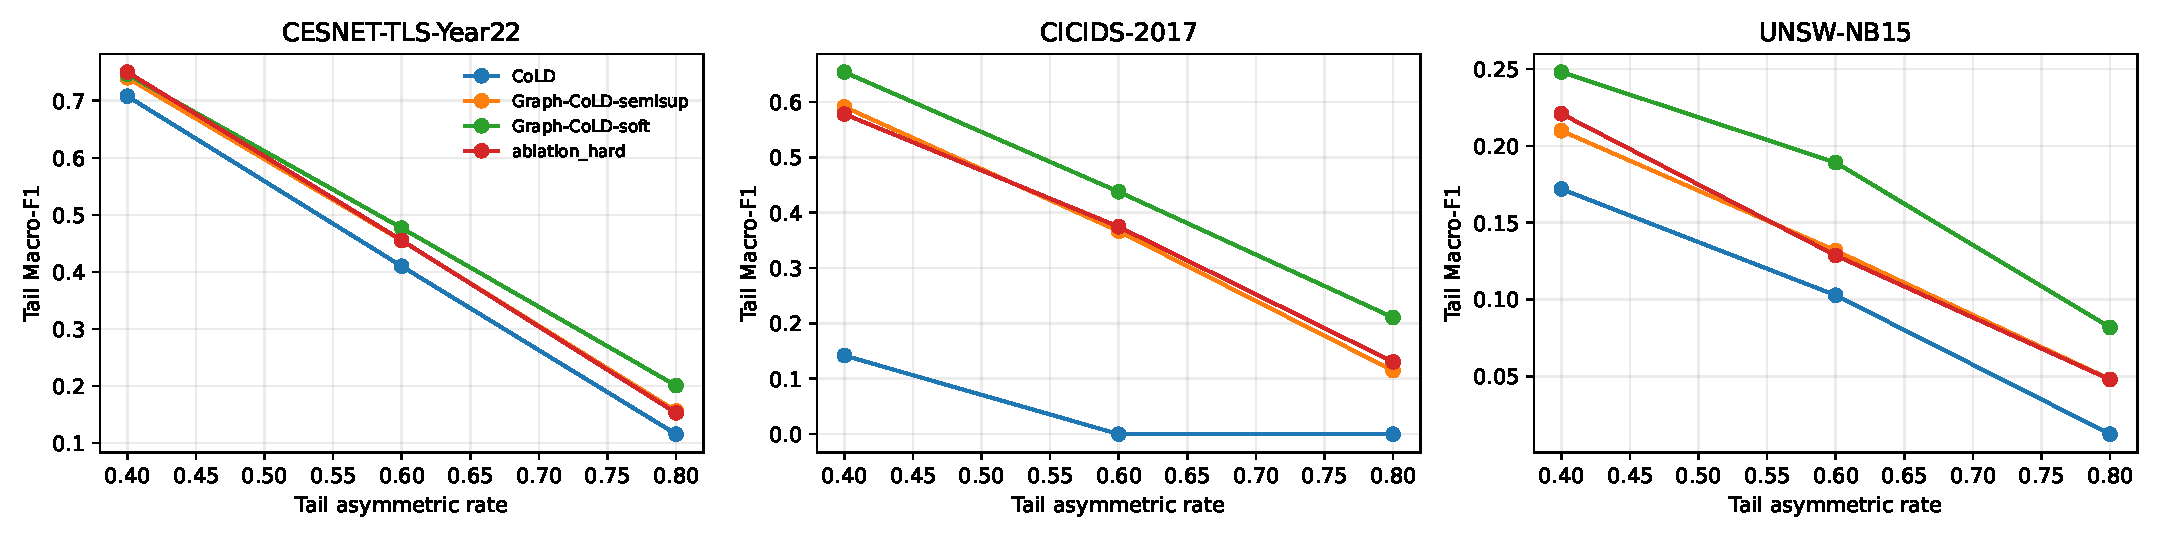
\includegraphics[width=0.98\linewidth]{fig_p2f_tail_powered.pdf}
\caption{Tail-class Macro-F1 of signal-preserving soft weighting vs.\ hard
deletion across asymmetric noise rates. The gain is small but consistent and
significant on all three datasets.}
\label{fig:tail}
\end{figure}

We stress an honesty point. An earlier ``rare-evidence recovery rate'' that counted
a sample as recovered whenever it was \emph{retained} was tautological. We redefine
recovery to require correct downstream classification; hard deletion is then no
longer automatically zero. Because soft retention still scores near-ceiling on
this diagnostic,\footnote{The secondary diagnostic values and its definition are
reported in \texttt{tables/table\_p2f\_summary.csv} and
\texttt{reports/p2f\_tighten.md}.} we rely solely on test-set tail-F1 for all
headline comparisons.

\paragraph{External anchors under the identical protocol.}
Table~\ref{tab:external} places two external noisy-label methods, run under the
identical P2f protocol (same audit windows, splits, seeds, and injected noise),
against Graph-CoLD-soft with scenario-paired tests. The ordering is consistent
across datasets. Confident Learning, a precise probabilistic pruner that removes
only 7--24\% of training rows, significantly outperforms Graph-CoLD-soft on
aggregate and tail metrics on all three datasets. The signal-preserving
weighting in turn outperforms hard deletion (Table~\ref{tab:tail}). Full
Co-Teaching collapses on tail classes (mean Tail-F1 $\approx 0$ at 60--80\%
noise on every dataset; \texttt{tables/table\_p5\_tail\_by\_rate.csv}), because
its small-loss forgetting systematically discards rare classes under this setup.
This result is specific to the evaluated implementation and does not establish a
general disadvantage of forgetting-based methods. Under the injected
tail-to-majority noise model, precise
pruning beats soft retention, because down-weighted flipped samples still teach
the classifier that tail features indicate the majority target. We therefore
scope the signal-retention claim to the mechanism level---within the shared
pipeline, soft weighting recovers rare classes that hard deletion loses---and we
identify Confident Learning as the performance bar that graph-based denoising
must clear; combining confident-learning-precision pruning with
graph-structured diagnostics is future work. Per-noise-rate tail-F1 breakdowns
for all methods are reported in \texttt{tables/table\_p5\_tail\_by\_rate.csv}.

\begin{table}[t]
\centering
\caption{External anchors vs.\ Graph-CoLD-soft under the identical P2f protocol:
scenario-paired mean differences ($n=30$ per dataset; positive $=$ external
method is better). All deltas shown are Holm-significant at $p<0.05$ in the
stated direction (Confident Learning above, Co-Teaching below Graph-CoLD-soft).
Source: \texttt{tables/table\_p5\_external\_tests.csv}.}
\label{tab:external}
\small
\begin{tabular}{llccc}
\toprule
Dataset & Method & $\Delta$Macro-F1 & $\Delta$Tail-F1 & $\Delta$Tail-recall \\
\midrule
\multirow{2}{*}{CICIDS-2017}
 & Confident-Learning & $+0.048$ & $+0.171$ & $+0.189$ \\
 & Co-Teaching & $-0.155$ & $-0.316$ & $-0.201$ \\
\midrule
\multirow{2}{*}{CESNET-TLS-Year22}
 & Confident-Learning & $+0.114$ & $+0.234$ & $+0.283$ \\
 & Co-Teaching & $-0.204$ & $-0.296$ & $-0.163$ \\
\midrule
\multirow{2}{*}{UNSW-NB15}
 & Confident-Learning & $+0.014$ & $+0.081$ & $+0.089$ \\
 & Co-Teaching & $-0.066$ & $-0.118$ & $-0.109$ \\
\bottomrule
\end{tabular}
\end{table}

\subsection{RQ3: A leakage audit prevents inflated claims}
\label{sec:res-leak}
Our initial pipeline reported a $\sim\!28$-point CICIDS advantage with a curve that
barely degraded under $60\%$ noise—implausible for a denoiser. Auditing revealed
that CICIDS-2017 contains $152{,}201/630{,}399$ ($\approx24\%$) exact-duplicate
training rows, and that any clean-label signal leaking into the score/graph
construction inflates results. We verified zero train/test edge crossings, removed
exact and near-duplicate edges, and eliminated the clean-label paths (enforced by a
regression test). The apparent advantage collapses to $+6.7$ points on CICIDS,
$+0.3$ on CESNET, and a slight $-1.3$ on UNSW in the audited comparison
(\texttt{reports/p2c\_leakage\_audit.md}). These audit deltas quantify the
magnitude of the inflation and were measured under the earlier P2c audit protocol
(a 3,000/8,000 stratified audit sample for CICIDS and the D5.5 frozen matrix for
CESNET/UNSW); they aggregate differently from, and are not directly comparable to,
the final P2f result matrix in Tables~\ref{tab:main}--\ref{tab:tail}
(\texttt{reports/p2f\_tighten.md}). We report this because graph denoising
in security is unusually susceptible to such inflation.

\subsection{RQ4: Graph informativeness is consistent with when the method helps}
\label{sec:res-info}
A per-dataset neighborhood-homophily / view-coverage diagnostic is directionally
consistent with
Graph-CoLD's margin: CICIDS (rich host/IP/temporal views) shows the largest gain,
CESNET sits near a performance ceiling, and UNSW (temporal/behavioral only) shows the
smallest—occasionally negative—margin
(Figure~\ref{fig:info}, \url{tables/table_p2d_graph_informativeness.csv}).
With only three datasets this pattern is descriptive, not inferential.
This turns the UNSW result into an informative boundary condition rather than a
failure: when views lack structural signal, the graph diagnostic adds little.

\begin{figure}[t]
\centering
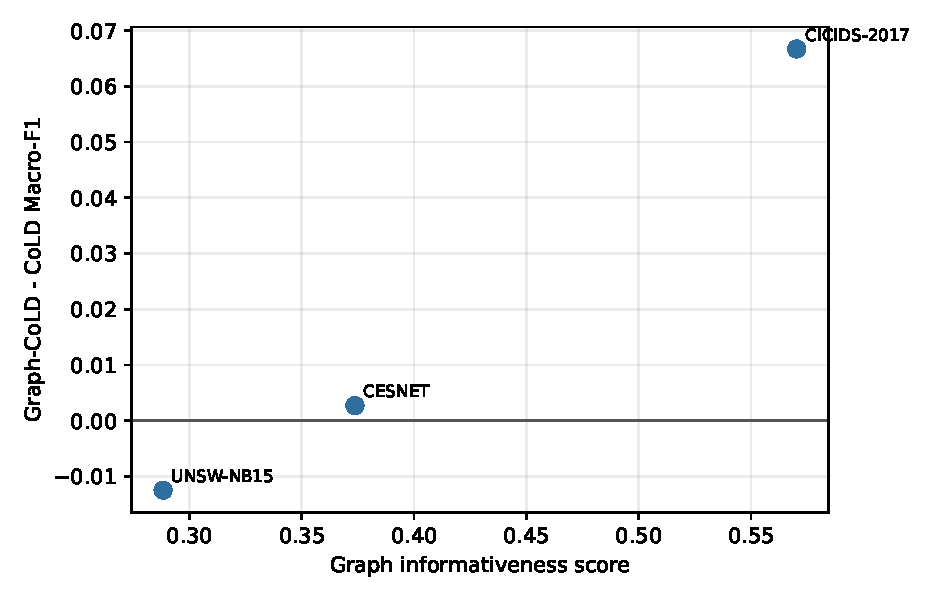
\includegraphics[width=0.9\linewidth]{fig_p2c_informativeness_margin.pdf}
\caption{Graph informativeness vs.\ Graph-CoLD margin over CoLD. Higher
neighborhood homophily and view coverage are directionally consistent with
larger gains (three datasets; descriptive pattern, not inferential).}
\label{fig:info}
\end{figure}

\subsection{RQ5: Cost}
Graph-CoLD's overhead is moderate: mean runtime is comparable to CoLD and memory
is lower than the strong purification baselines (the runtime and memory figures
are measured under the earlier D5.5-protocol runs recorded in
\texttt{results/runtime.json}; the relative pattern, not the absolute numbers, is
the claim). Signal preservation adds
negligible cost over hard deletion because it changes only the training weights.

\section{Discussion}
\label{sec:discuss}
% <<P4-DISCUSSION>>
% BLOCK D -> <<P4-DISCUSSION>>

The operational motivation is strongest in settings where multiple telemetry
sources provide partially consistent signals, such as host relationships,
communication patterns, and temporal behavior. In those settings, a suspicious
sample need not be useless: a rare attack instance may appear inconsistent
because it represents an emerging technique rather than an incorrect label. Our
benchmark study tests only this training-data mechanism; it does not establish
deployment suitability.

However, the results also demonstrate clear boundaries. When available views
are weak or incomplete, graph structure provides limited additional information.
The UNSW-NB15 results illustrate this condition: without sufficiently
informative relational views, graph-based diagnostics cannot reliably create
additional training signal. Similarly, datasets operating near a performance ceiling,
such as CESNET-TLS-Year22 under the evaluated protocol, naturally limit the
observable improvement.

A key methodological decision in this work is the avoidance of unfair
state-of-the-art comparisons. Two external anchors---Confident Learning and a
full Co-Teaching implementation---were therefore run under the identical
leakage-audited protocol and are reported in Table~\ref{tab:external}, even
though one of them outperforms our method on every dataset; that result is part
of the empirical record, not an inconvenience. Other purification and robust-training
variants (MCRe, MORSE, FINE, Decoupling) were not all
reimplemented under the final leakage-audited protocol. Mixing results obtained
under different data-cleaning, duplication-removal, and evaluation settings
would create an unreliable comparison, so those methods remain excluded from
the formal matrix. A comprehensive comparison with all previous methods
requires faithful implementations or official code under a unified evaluation
framework.

The external-anchor ordering carries a practical lesson for benchmark data
curation and a hypothesis for later SOC-facing validation.
Confident Learning's precise pruning---removing only 7--24\% of rows---sets the
performance bar under the injected noise model, while the evaluated Co-Teaching
configuration nearly eliminates the tail classes. The
differentiator is not deletion versus retention but \emph{diagnostic precision}:
an imprecise purifier can sacrifice scarce rare-class training signal, whether
it deletes samples or down-weights mislabeled samples insufficiently. Combining
confident-learning-precision pruning with
graph-structured diagnostics is the natural next step.

The leakage audit provides a broader methodological lesson for graph-based
security machine learning. Graph models can unintentionally exploit duplicated
records, cross-split connections, or hidden clean-label information. Such
effects may produce impressive but misleading improvements. Therefore, graph
security studies should explicitly verify data separation, graph construction
constraints, and label independence before reporting performance gains.

Future work should extend Graph-CoLD toward streaming SOC environments,
full-archive evaluation, analyst-in-the-loop validation, and broader
cross-domain benchmark comparisons. These extensions are necessary to determine
whether signal-preserving denoising remains effective when labels arrive
continuously and attack distributions evolve over time.
The results support a bounded but useful claim. A label-space graph diagnostic
modestly improves noisy-label IDS over CoLD where views are informative, and—more
distinctively—signal-preserving weighting retains rare-class training examples
that hard deletion discards, improving Tail-F1 under high asymmetric noise within
the shared pipeline. The current analysis detects no significant aggregate
difference but does not establish equivalence. Under the same protocol,
confident-learning pruning remains the stronger performer and marks the bar for
future graph-based denoisers. We deliberately avoid three overclaims that our own experiments
do not support: a universal accuracy advantage (the aggregate gain is modest and
largely from the graph, not the weighting), a ranking advantage (Graph-CoLD
ties strong peers on top-$K$ precision), or SOC/forensic effectiveness from
benchmark-level sample retention.

\section{Threats to Validity}
\label{sec:threats}
\emph{Internal.} The evaluation uses deterministic audit windows for tractability;
absolute Macro-F1 is therefore lower than full-archive runs, though the paired,
seed-controlled comparisons are the object of inference. MCRe and MORSE pass a
clean-label sanity floor but degrade on high-noise tabular settings more than in
their original domains; we report this caveat rather than a possibly unfaithful
number (\texttt{reports/p2b\_baseline\_fidelity.md}).
\emph{Construct.} The rare-evidence-recovery diagnostic, even after correction,
saturates for soft retention; we therefore headline test-set tail-F1.
\emph{External.} CICIDS-2017, CESNET-TLS-Year22, and UNSW-NB15 are useful
benchmarks but not complete SOC deployments; the priority score is evaluated by
proxy, not an analyst study. The two-dataset lock recorded in the D9 submission
audit was an intermediate checkpoint; the authoritative final scope is the
three-dataset P2f clean de-oracled protocol.

\section{Limitations}
\label{sec:limits}
MALTLS-22 and OpTC are not evaluated (no verified license/provenance path).
Behavioral and threat-intelligence views are disabled where fields are absent. The
aggregate accuracy contribution is modest and dataset-dependent; under the
audited protocol, Confident Learning outperforms Graph-CoLD on aggregate and
tail metrics on all three datasets, so the distinctive contribution is the
leakage audit, the mechanism-level signal-retention finding, and the
informativeness boundary analysis rather than state-of-the-art accuracy.
Full-archive and streaming
evaluations are left to future work.

\section{Conclusion}
\label{sec:conclusion}
We revisited collaborative label denoising and asked whether a multi-view
label-space graph diagnostic and signal-preserving weighting improve robustness.
The answer is targeted: the graph diagnostic gives a modest,
informativeness-dependent accuracy gain over CoLD, and signal-preserving weighting
improves Tail-F1 over hard deletion under high asymmetric noise within the shared
pipeline. The current aggregate analysis detects no significant difference but
does not establish equivalence. A confident-learning anchor, evaluated under the
identical protocol, outperforms both. Alongside, we
contribute a leakage audit and a graph-informativeness diagnostic that together
explain when—and when not—graph denoising helps. More broadly, our results
argue that security data curation should shift from indiscriminate purification
toward signal-aware retention, in which deletion decisions explicitly weigh
the class-level cost of discarding scarce training examples against the precision
of the noise diagnostic. CESNET supports only a service-class stress-test claim;
attack-level conclusions are limited to CICIDS and UNSW. We hope the audit, and the
audited external-baseline ordering, are as useful to the community as the method.

\begin{appendices}
\section{CESNET-TLS-Year22 class-filter policy}
\label{app:cesnet-policy}
\renewcommand{\thetable}{A\arabic{table}}
\renewcommand{\theHtable}{A.\arabic{table}}
CESNET is evaluated as a TLS service-classification stress test, not as an attack
dataset. The repository audit report
\texttt{reports/cesnet\_class\_policy\_report.json} records 178 raw service labels.
The frozen post-filter policy retains the 25 labels in Table~\ref{tab:cesnet-policy}
because each has at least 1,000 rows in the audited source window; the other 153
labels are excluded rather than merged. The largest retained class is capped at
4,958 rows. Counts below are pre-split source-window counts and are not labels of
attack prevalence.

\begin{table}[ht]
\centering
\caption{Frozen CESNET 178-to-25 service-class filter.}
\label{tab:cesnet-policy}
\footnotesize
\begin{tabular}{lr@{\qquad}lr}
\hline
Service label & Count & Service label & Count \\
\hline
apple-itunes & 1,666 & bitdefender-gravityzone & 1,943 \\
dropbox & 2,472 & eset-edf & 1,506 \\
eset-edtd & 1,324 & facebook-graph & 1,989 \\
google-www & 1,088 & instagram & 1,323 \\
kaspersky & 1,459 & microsoft-authentication & 3,083 \\
microsoft-defender & 1,326 & microsoft-diagnostic & 4,958 \\
microsoft-onedrive & 3,137 & microsoft-push & 3,516 \\
microsoft-settings & 4,808 & microsoft-update & 4,958 \\
o2tv & 1,989 & office365 & 2,584 \\
outlook & 3,517 & seznam-media & 1,787 \\
skype & 3,511 & spotify & 1,217 \\
teams & 3,802 & tiktok & 1,128 \\
vmware-vcsa & 1,033 & & \\
\hline
\end{tabular}
\end{table}
\end{appendices}

%% ------------------------------------------------------------------
\begin{thebibliography}{99}
\bibitem{yang2026cold} S. Yang, X. Zheng, J. Li, J. Xu, E. C. H. Ngai,
CoLD: Collaborative label denoising framework for network intrusion detection,
in: Network and Distributed System Security (NDSS) Symposium, 2026.
Available: \url{https://dx.doi.org/10.14722/ndss.2026.231950}
\bibitem{arp2022dodont} D. Arp et al., Dos and don'ts of machine learning in
computer security, in: USENIX Security Symposium, 2022, pp. 3971--3988.
\bibitem{song2022survey} H. Song, M. Kim, D. Park, Y. Shin, J.-G. Lee,
Learning from noisy labels with deep neural networks: A survey,
IEEE TNNLS 34 (11) (2022) 8135--8153.
\bibitem{patrini2017making} G. Patrini, A. Rozza, A. K. Menon, R. Nock, L. Qu,
Making deep neural networks robust to label noise: A loss correction approach,
in: CVPR, 2017, pp. 1944--1952.
\bibitem{han2018coteaching} B. Han et al., Co-teaching: Robust training of deep
neural networks with extremely noisy labels, in: NeurIPS, 2018, pp. 8535--8545.
\bibitem{yu2019coteachingplus} X. Yu et al., How does disagreement help
generalization against label corruption?, in: ICML, 2019, pp. 7164--7173.
\bibitem{malach2017decoupling} E. Malach, S. Shalev-Shwartz, Decoupling ``when to
update'' from ``how to update'', in: NeurIPS, 2017, pp. 960--970.
\bibitem{li2020dividemix} J. Li, R. Socher, S. C. H. Hoi, DivideMix: Learning with
noisy labels as semi-supervised learning, in: ICLR, 2020.
\bibitem{northcutt2021confident} C. G. Northcutt, L. Jiang, I. L. Chuang,
Confident learning: Estimating uncertainty in dataset labels,
JAIR 70 (2021) 1373--1411.
\bibitem{kim2021fine} T. Kim, J. Ko, J. Choi, S.-Y. Yun, FINE samples for learning
with noisy labels, in: NeurIPS, 2021, pp. 24137--24149.
\bibitem{wu2023morse} X. Wu, W. Guo, J. Yan, B. Coskun, X. Xing, From grim reality
to practical solution: Malware classification in real-world noise, in: IEEE S\&P,
2023, pp. 2602--2619.
\bibitem{yuan2023mcre} Q. Yuan, G. Gou, Y. Zhu, Y. Zhu, G. Xiong, Y. Wang,
MCRe: A unified framework for handling malicious traffic with noise labels,
IEEE Transactions on Information Forensics and Security, 2023.
\bibitem{kipf2017gcn} T. N. Kipf, M. Welling, Semi-supervised classification with
graph convolutional networks, in: ICLR, 2017.
\bibitem{velickovic2018gat} P. Veli\v{c}kovi\'c et al., Graph attention networks,
in: ICLR, 2018.
\bibitem{hamilton2017graphsage} W. L. Hamilton, R. Ying, J. Leskovec, Inductive
representation learning on large graphs, in: NeurIPS, 2017.
\bibitem{hu2020hgt} Z. Hu, Y. Dong, K. Wang, Y. Sun, Heterogeneous graph
transformer, in: The Web Conference (WWW), 2020, pp. 2704--2710.
\bibitem{chen2020simclr} T. Chen, S. Kornblith, M. Norouzi, G. Hinton, A simple
framework for contrastive learning of visual representations, in: ICML, 2020,
pp. 1597--1607.
\bibitem{rehman2024flash} M. U. Rehman, H. Ahmadi, W. U. Hassan, Flash: A
comprehensive approach to intrusion detection via provenance graph representation
learning, in: IEEE S\&P, 2024, pp. 3552--3570.
\bibitem{xu2024argus} J. Xu, X. Shu, Z. Li, Understanding and bridging the gap
between unsupervised network representation learning and security analytics, in:
IEEE S\&P, 2024, pp. 3590--3608.
\bibitem{yang2021cade} L. Yang et al., CADE: Detecting and explaining concept
drift samples for security applications, in: USENIX Security Symposium, 2021,
pp. 2327--2344.
\bibitem{vaarandi2024nids} R. Vaarandi, A. Guerra-Manzanares, Network IDS alert
classification with active learning techniques, Journal of Information Security
and Applications 81 (2024) 103687.
\bibitem{chavali2024rlalert} L. Chavali, A. Krishnan, P. Saxena, B. Mitra,
A. Sreevallabh Chivukula, Off-policy actor-critic deep reinforcement learning for
alert prioritization in intrusion detection systems, Computers \& Security 142
(2024) 103854.
\bibitem{sharafaldin2018cicids} I. Sharafaldin, A. H. Lashkari, A. A. Ghorbani,
Toward generating a new intrusion detection dataset and intrusion traffic
characterization, in: ICISSP, 2018, pp. 108--116.
\bibitem{hynek2024cesnet} K. Hynek, J. Luxemburk, J. Pesek, T. Cejka, P. Siska,
CESNET-TLS-Year22: A year-spanning TLS network traffic dataset from backbone
lines, Scientific Data 11 (2024) 1156.
\bibitem{moustafa2015unsw} N. Moustafa, J. Slay, UNSW-NB15: A comprehensive data
set for network intrusion detection systems, in: Military Communications and
Information Systems Conference (MilCIS), 2015, pp. 1--6.
\bibitem{guerra2022datasets} J. L. Guerra, C. Catania, E. Veas, Datasets are not
enough: Challenges in labeling network traffic, Computers \& Security 120
(2022) 102810.
\bibitem{qing2023lowquality} Y. Qing et al., Low-quality training data only? A
robust framework for detecting encrypted malicious network traffic, arXiv
preprint arXiv:2309.04798, 2023.
\bibitem{zhao2021enhancing} Z. Zhao et al., Enhancing robustness of on-line
learning models on highly noisy data, IEEE TDSC 18 (5) (2021) 2177--2192.
\bibitem{wang2022feco} N. Wang et al., FeCo: Boosting intrusion detection
capability in IoT networks via contrastive learning, in: IEEE INFOCOM, 2022,
pp. 1409--1418.
\bibitem{yue2022cleid} Y. Yue et al., Contrastive learning enhanced intrusion
detection, IEEE TNSM 19 (4) (2022) 4232--4247.
\bibitem{liu2025deepdrac} Y. Liu et al., DeepDRAC: Disposition recommendation
for alert clusters based on security event patterns, IEEE TIFS 20 (2025)
6443--6458.
\bibitem{shon2023semisup} H. G. Shon, Y. Lee, M. Yoon, Semi-supervised alert
filtering for network security, Electronics 12 (23) (2023) 4755.
\bibitem{wang2024alertagg} W. Wang et al., Transformer-based framework for
alert aggregation and attack prediction in a multi-stage attack, Computers
\& Security 136 (2024) 103533.
\bibitem{xia2021sample} X. Xia et al., Sample selection with uncertainty of
losses for learning with noisy labels, arXiv preprint arXiv:2106.00445, 2021.
\bibitem{liu2021metric} C. Liu et al., Noise-resistant deep metric learning with
ranking-based instance selection, in: CVPR, 2021, pp. 6811--6820.
\bibitem{yang2024recda} S. Yang et al., RecDA: Concept drift adaptation with
representation enhancement for network intrusion detection, in: ACM SIGKDD,
2024, pp. 3818--3828.
\bibitem{andresini2021insomnia} G. Andresini et al., Insomnia: Towards
concept-drift robustness in network intrusion detection, in: ACM AISec, 2021,
pp. 111--122.
\bibitem{hynek2024zenodo} K. Hynek et al., CESNET-TLS-Year22 dataset, Zenodo
record 10608607, 2024.
\bibitem{moustafa2016unsw} N. Moustafa, J. Slay, The evaluation of network
anomaly detection systems: UNSW-NB15, Information Security Journal 25 (1--3)
(2016) 18--31.
\end{thebibliography}
\end{document}
